\documentclass[tikz,border=5pt]{standalone}
\usepackage{ctex,amsmath}
\usetikzlibrary{arrows.meta,calc}
\tikzset{>=Latex,membrane/.style={blue!65!black,thick},force/.style={orange!85!black,thick,->},axis/.style={gray,->}}
\begin{document}
\begin{tikzpicture}[font=\small]
\begin{scope}
\shade[top color=blue!4,bottom color=blue!18](0,0)circle[radius=1.25];
\draw[membrane](0,0)circle[radius=1.25];
\draw[gray,dashed](0,0)circle[radius=1.05];
\draw[membrane,dashed](-1.25,0)arc[start angle=180,end angle=0,x radius=1.25,y radius=.24];
\draw[membrane](-1.25,0)arc[start angle=180,end angle=360,x radius=1.25,y radius=.24];
\draw[blue!35](0,0)ellipse[x radius=.32,y radius=1.25];
\fill(0,0)circle[radius=.025];
\draw[->](0,0)--({1.25*cos(35)},{1.25*sin(35)})node[midway,above left]{$r$};
\draw[gray,->](0,0)--({1.05*cos(-40)},{1.05*sin(-40)})node[midway,below left,text=black]{$r_0$};
\node[below]at(0,-1.65){$r=r_0+\Delta r$};
\end{scope}
\begin{scope}[xshift=4.5cm]
\shade[top color=blue!6,bottom color=blue!22](1.35,0)arc[start angle=0,end angle=180,radius=1.35]--cycle;
\draw[membrane](1.35,0)arc[start angle=0,end angle=180,radius=1.35];
\draw[gray,dashed](-1.35,0)arc[start angle=180,end angle=0,x radius=1.35,y radius=.23];
\draw[membrane](-1.35,0)arc[start angle=180,end angle=360,x radius=1.35,y radius=.23];
\draw[force](0,.22)--(0,1.08);
\node[above]at(0,1.65){$\Delta p\,\pi r^2$};
\draw[force](-.94,-.15)--(-.94,-.90);
\draw[force](.94,-.15)--(.94,-.90);
\node[below]at(-.94,-.95){$\sigma\,\mathrm d\ell$};
\node[below]at(.94,-.95){$\sigma\,\mathrm d\ell$};
\draw[gray,->](0,0)--(1.35,0)node[midway,below,text=black]{$r$};
\node[below]at(0,-1.65){切口周长$2\pi r$};
\end{scope}
\end{tikzpicture}
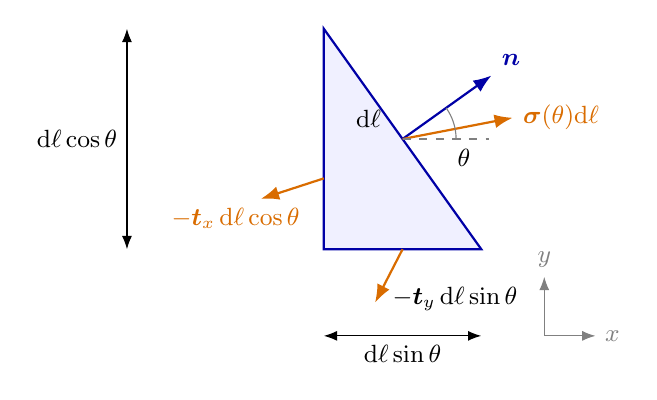
\begin{tikzpicture}[font=\small]
\fill[blue!6](0,0)--(2,0)--(0,2.8)--cycle;
\draw[membrane](0,0)--(2,0)--(0,2.8)--cycle;
\draw[force](0,.9)--(-.8,.64);
\node[below,text=orange!85!black]at(-1.12,.64){$-\boldsymbol t_x\,\mathrm d\ell\cos\theta$};
\draw[force](1,0)--(.65,-.68);
\node[right]at(.75,-.63){$-\boldsymbol t_y\,\mathrm d\ell\sin\theta$};
\draw[blue!65!black,thick,->](1,1.4)--(2.13,2.207)node[above right]{$\boldsymbol n$};
\draw[force](1,1.4)--(2.4,1.67)node[right]{$\boldsymbol\sigma(\theta)\mathrm d\ell$};
\draw[gray,dashed](1,1.4)--(2.1,1.4);
\draw[gray](1.68,1.4)arc[start angle=0,end angle=35.54,radius=.68];
\node[below]at(1.78,1.4){$\theta$};
\node[left]at(.85,1.65){$\mathrm d\ell$};
\draw[<->](-2.5,0)--(-2.5,2.8)node[midway,left]{$\mathrm d\ell\cos\theta$};
\draw[<->](0,-1.1)--(2,-1.1)node[midway,below]{$\mathrm d\ell\sin\theta$};
\draw[axis](2.8,-1.1)--(3.45,-1.1)node[right]{$x$};
\draw[axis](2.8,-1.1)--(2.8,-.35)node[above]{$y$};
\end{tikzpicture}
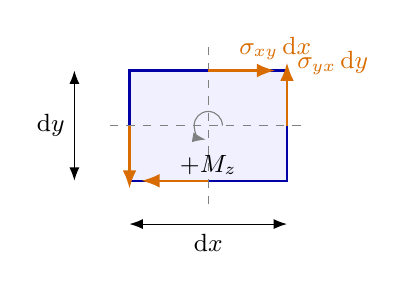
\begin{tikzpicture}[font=\small]
\fill[blue!6](-1,-.7)rectangle(1,.7);
\draw[membrane](-1,-.7)rectangle(1,.7);
\draw[gray,dashed](-1.25,0)--(1.25,0)(0,-1)--(0,1);
\draw[force](0,.7)--(.85,.7)node[above]{$\sigma_{xy}\,\mathrm dx$};
\draw[force](0,-.7)--(-.85,-.7);
\draw[force](1,0)--(1,.8)node[right]{$\sigma_{yx}\,\mathrm dy$};
\draw[force](-1,0)--(-1,-.8);
\draw[<->](-1,-1.25)--(1,-1.25)node[midway,below]{$\mathrm dx$};
\draw[<->](-1.7,-.7)--(-1.7,.7)node[midway,left]{$\mathrm dy$};
\draw[gray,->](.18,0)arc[start angle=0,end angle=260,radius=.18];
\node[below]at(0,-.25){$+M_z$};
\end{tikzpicture}
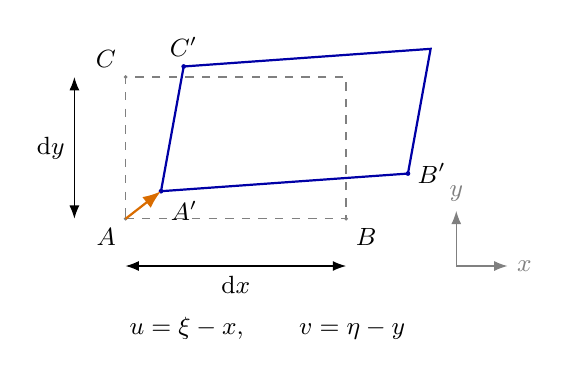
\begin{tikzpicture}[font=\small]
\coordinate(A)at(0,0);\coordinate(B)at(2.8,0);\coordinate(C)at(0,1.8);
\coordinate(Ap)at(.45,.35);\coordinate(Bp)at(3.586,.574);\coordinate(Cp)at(.738,1.934);
\draw[gray,dashed](A)--(B)--(2.8,1.8)--(C)--cycle;
\draw[membrane](Ap)--(Bp)--(3.874,2.158)--(Cp)--cycle;
\foreach \pt in {A,B,C}\fill[gray](\pt)circle[radius=.025];
\foreach \pt in {Ap,Bp,Cp}\fill[blue!65!black](\pt)circle[radius=.03];
\node[below left]at(A){$A$};\node[below right]at(B){$B$};\node[above left]at(C){$C$};
\node[below right]at(Ap){$A'$};\node[right]at(Bp){$B'$};\node[above]at(Cp){$C'$};
\draw[force](A)--(Ap);
\draw[<->](0,-.60)--(2.8,-.60)node[midway,below]{$\mathrm dx$};
\draw[<->](-.65,0)--(-.65,1.8)node[midway,left]{$\mathrm dy$};
\draw[axis](4.2,-.60)--(4.85,-.60)node[right]{$x$};
\draw[axis](4.2,-.60)--(4.2,.10)node[above]{$y$};
\node[below]at(1.8,-1.12){$u=\xi-x,\qquad v=\eta-y$};
\end{tikzpicture}
\end{document}
